\chapter{Resultados e Discussão}\label{cap:resultados}

\section{Desafio em trajeto específico dificuldade fácil}
Aqui o treino foi feito em dois trajetos (identificados por \textit{Path(0)} e \textit{Path(8)} no projeto), ambos exigem que o agente faça uma conversão do veículo (ver Figura \ref{fig:trajetos-desafio-facil}). O primeiro exige que o agente faça uma curva à esquerda e siga reto até o destino, o outro exige o agente siga reto e faça uma conversão à direita.

\begin{figure}[h]
    \centering
    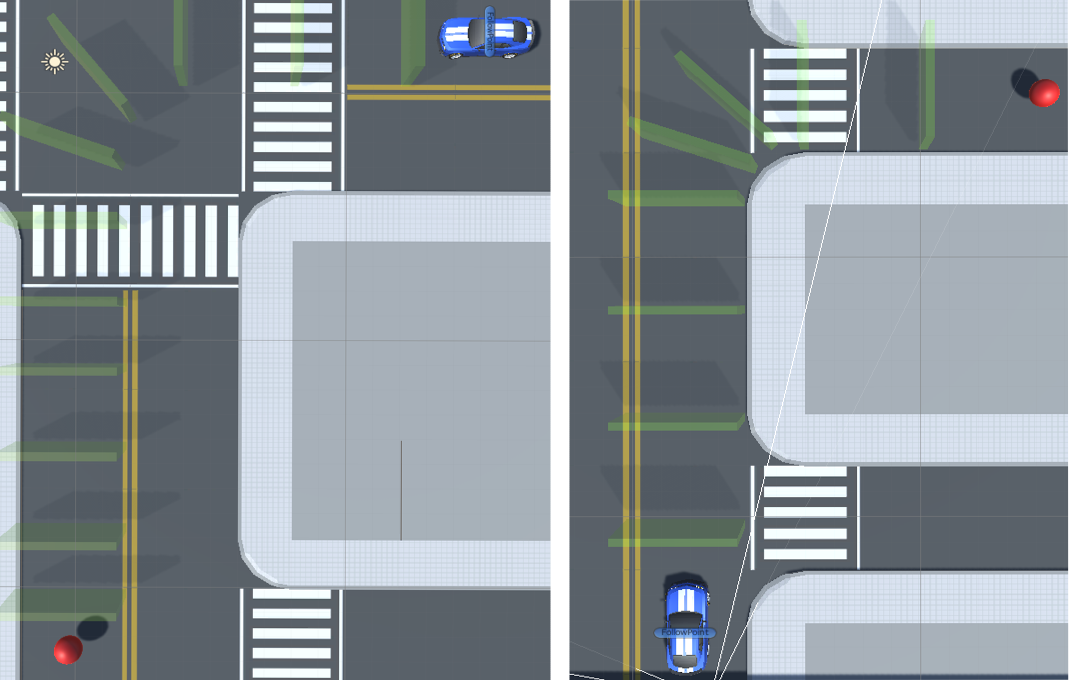
\includegraphics{figs/treinos/desafio-mediano/paths_0-8.png}
    \caption{Trajetos deste desafio, à esquerda o \textit{Path(0)} e à direita o \textit{Path(8)}.}
    \label{fig:trajetos-desafio-facil}
\end{figure}

\begin{figure}[h]
    \centering
    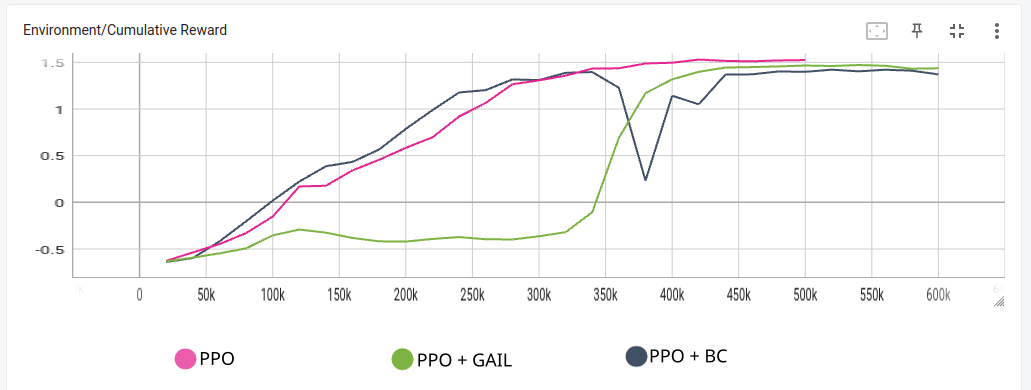
\includegraphics[scale=0.42]{figs/treinos/desafio-mediano/path0/recompensa-ppo-bc-gail-path0.png}
    \caption{Recompensa cumulativa mediana por \textit{steps} durante o treino do agente no \textit{} Path(0).}
    \label{fig:result-desafio-1-path-0}
\end{figure}

\begin{figure}[h]
    \centering
    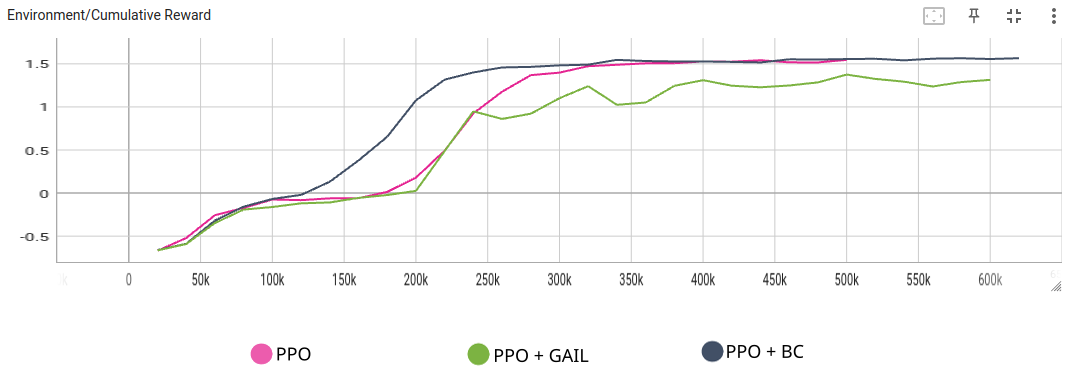
\includegraphics[scale=0.42]{figs/treinos/desafio-mediano/path8/recompensa-ppo-bc-gail-path8.png}
    \caption{Recompensa cumulativa mediana por \textit{steps} durante o treino do agente no \textit{Path(8)}.}
    \label{fig:result-desafio-1-path-8}
\end{figure}

O treinamento não encontrou problemas para convergir neste desafio em qualquer dos três algoritmos. PPO foi o que obteve a melhor mediana final no \textit{Path(0)} mesmo dispondo de menos \textit{steps} para treinar (identificado pela linha rosa nas Figuras \ref{fig:result-desafio-1-path-0} e \ref{fig:result-desafio-1-path-8}). Embora tenham convergido no \textit{Path(0)}, GAIL e BC se mostraram instáveis. O primeiro demorou muito para mostrar algum progresso na recompensa, enquanto BC apresentou uma anomalia após 350 mil \textit{steps} voltando a se estabilizar após 450 mil passos, como mostra a Figura \ref{fig:result-desafio-1-path-0}. Quanto ao \textit{Path(8)}, o treino que utilizou BC convergiu mais rápido que o de PPO e também obteve uma mediana maior que este. Neste trajeto o GAIL foi o mais instável, o único que não convergiu (linha verde da Figura \ref{fig:result-desafio-1-path-8}).

\begin{table}[htpb]
    \centering
    \caption{Consolidado de resultados por rota e algoritmo, contém a mediana final da recompensa no treino, a coluna de desempenho teste é quantas rotas completou de quantas tentativas e média de recompensas nos testes.}
    \label{resultado-tabela-desafio-1}
    \begin{tabular}{|l|c|c|c|c|c|c|r|}
         \hline
         \small{Rota}                         & \small{Algoritmo}   & \small{Mediana final rec. Treino}  & \small{Desempenho teste}    & \small{Média rec. Testes}  \\ \hline
         \multirow{3}{*}{\textit{Path(0)}}    &      PPO            &   1.524                            &    10/10                     &      1                    \\ \cline{2-5}
                                              &      GAIL           &   1.436                            &    10/10                     &      1                    \\ \cline{2-5}
                                              &      BC             &   1.371                            &    10/10                     &      1                    \\ \hline
         \multirow{3}{*}{\textit{Path(8)}}    &      PPO            &   1.546                            &    10/10                     &      1                    \\ \cline{2-5}
                                              &      GAIL           &   1.314                            &    6/10                      &      0.585                \\ \cline{2-5}
                                              &      BC             &   1.565                            &    10/10                     &      1                    \\ \hline
    \end{tabular}
\end{table}


Nos testes, com exceção do algoritmo GAIL no \textit{Path(8)}, todos os agentes desempenharam a tarefa sem falha alguma. O  cérebro treinado com o algoritmo BC subiu na calçada uma vez em cada teste, mas a punição por uma ocorrência não é suficiente para afetar sua média. O agente treinado com GAIL no \textit{Path(8)} falhou em 4 dos 10 testes, não há certeza do porque disto, mas talvez seu desempenho foi afetado porque a rota 8 exige que a curva seja feita após percorrer um trajeto reto, o contrário do \textit{Path(0)}, que exige que a curva seja feita logo após o ponto de partida. Esta exigência de mudança no comportamento do agente pode ser a causa do GAIL ter falhado.

\section{Desafio em trajeto específico difícil}
Para este desafio foi testado em três rotas diferentes: \textit{Path(3), Path(5) e Path(6)}. A Figura \ref{fig:trajetos-desafio-dificil} exibe a visão superior dos três trajetos. O primeiro é o mais complexo possuindo três curvas alternadas, enquanto \textit{Path(5)} requer que o carro faça duas conversões à direita e o último trajeto contém duas curvas alternadas. 

\begin{figure}[h]
    \centering
    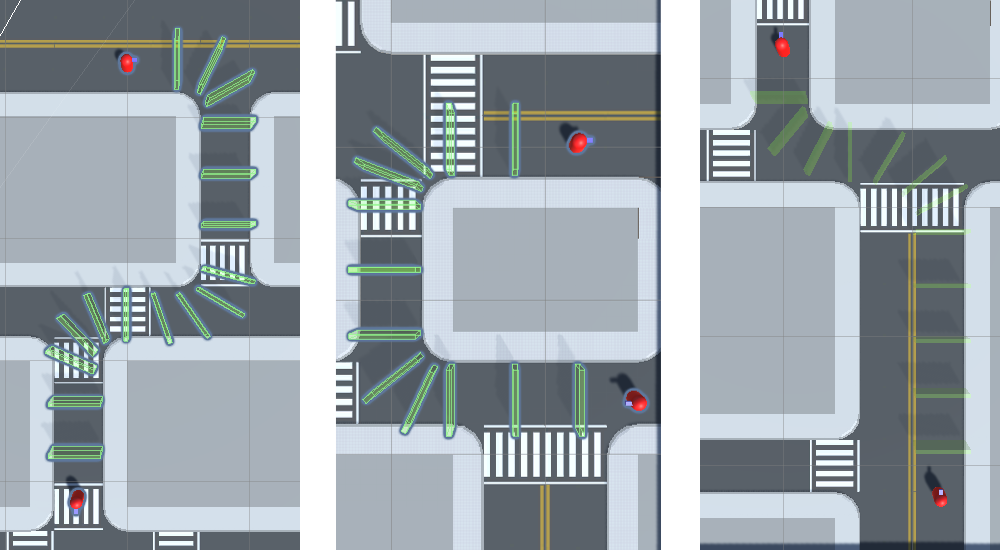
\includegraphics{figs/treinos/desafio-dificil/rotas.png}
    \caption{Visão superior das três rotas do desafio específico difícil.}
    \label{fig:trajetos-desafio-dificil}
\end{figure}

Neste desafio, a diferença do resultado dos treinos entre os algoritmos aumentou. Na Figura \ref{fig:result-desafio-2-path-3} pode-se notar que apenas o PPO foi estável e convergiu no \textit{Path(3)}, enquanto BC a partir da metade do treino passou a perder a recompensa, ficando preso em um mínimo local. O mesmo ocorreu com GAIL, porém este não chegou a apresentar progresso em momento algum. 

\begin{figure}[h]
    \centering
    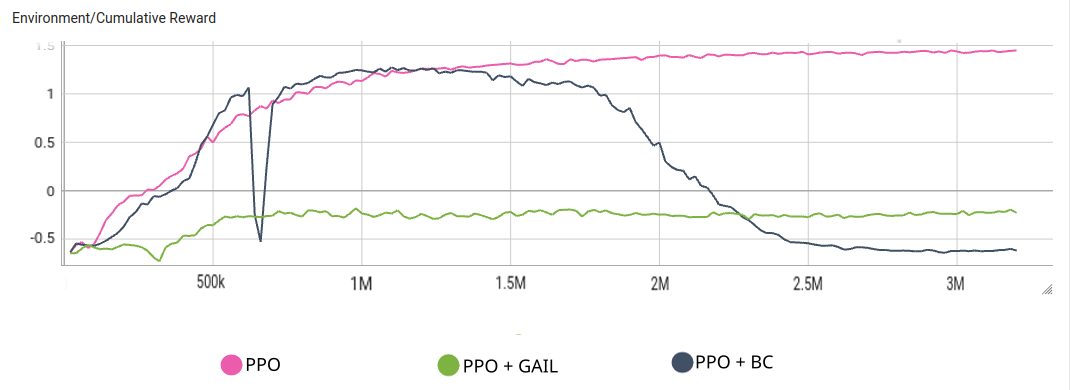
\includegraphics[scale=0.35]{figs/treinos/desafio-dificil/path-3_recompensas-algos.png}
    \caption{Recompensa cumulativa mediana por \textit{steps} durante o treino do agente no \textit{Path(3)}.}
    \label{fig:result-desafio-2-path-3}
\end{figure}

No \textit{Path(5)}, que exige duas curvas à esquerda, PPO e BC convergiram rapidamente, com BC se mantendo estável desta vez. GAIL, por outro lado, ficou preso em um mínimo local, mesmo dispondo de mais \textit{steps} que os outros, não conseguiu apresentar melhora (ver Figura \ref{fig:result-desafio-2-path-5}).

\begin{figure}[h]
    \centering
    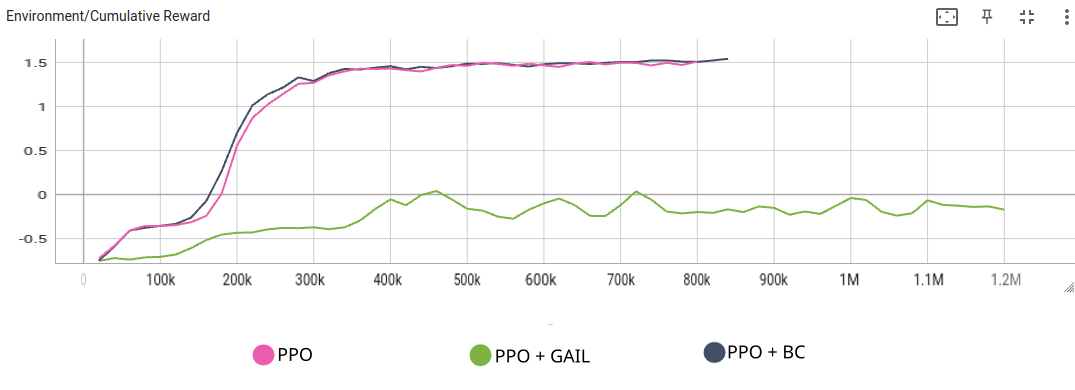
\includegraphics[scale=0.35]{figs/treinos/desafio-dificil/path-5_recompensas-algos.png}
    \caption{Recompensa cumulativa mediana por \textit{steps} durante o treino do agente no \textit{Path(5)}.}
    \label{fig:result-desafio-2-path-5}
\end{figure}

\begin{figure}[h]
    \centering
    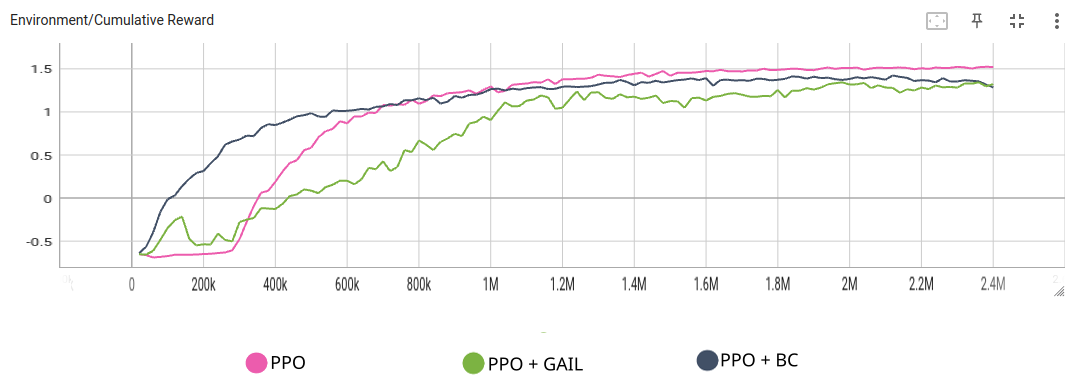
\includegraphics[scale=0.35]{figs/treinos/desafio-dificil/path-6_recompensas-algos.png}
    \caption{Recompensa cumulativa mediana por \textit{steps} durante o treino do agente no \textit{Path(6)}.}
    \label{fig:result-desafio-2-path-6}
\end{figure}

No \textit{Path(6)}, os três algoritmos apresentaram uma melhora constante e estável nos treinos. Na Figura \ref{fig:result-desafio-2-path-6}, é possível ver que apesar de o PPO ter obtido uma melhor mediana final (linha rosa na Figura), o BC teve um aprendizado mais rápido inicialmente (linha preta). Neste trajeto, GAIL também se mostrou mais instável que os demais, porém obteve um desempenho melhor aqui que noutros trajetos, inclusive com uma mediana final ligeiramente acima de BC no \textit{Path(6)}.

\begin{table}[htpb]
    \centering
    \caption{Consolidado de resultados por rota e algoritmo do segundo desafio.}
    \label{resultado-tabela-desafio-2}
    \begin{tabular}{|l|c|c|c|c|c|c|r|}
         \hline
         \small{Rota} & \small{Algoritmo}   & \small{Mediana final rec. Treino}  & \small{Desempenho testes}    & \small{Média rec. Testes}                       \\ \hline
         \multirow{3}{*}{\textit{Path(3)}}  &      PPO            &   1,449                            &    10/10                     &      0,97                 \\ \cline{2-5}
                                            &      GAIL           &   -0,229                           &    0/10                      &      -0,261               \\ \cline{2-5}
                                            &      BC             &   -0,618                           &    0/10                      &      -0.693               \\ \hline
         \multirow{3}{*}{\textit{Path(5)}}  &      PPO            &   1,509                            &    10/10                     &      0,98                 \\ \cline{2-5}
                                            &      GAIL           &   -0,171                           &    0/10                      &      -0,252               \\ \cline{2-5}
                                            &      BC             &   1,505                            &    10/10                     &      1                    \\ \hline
         \multirow{3}{*}{\textit{Path(6)}}  &      PPO            &   1,522                            &    10/10                     &      0,993                \\ \cline{2-5}
                                            &      GAIL           &   1,323                            &    10/10                     &      0,99                 \\ \cline{2-5}
                                            &      BC             &   1,284                            &    5/10                      &      0,42                 \\ \hline
    \end{tabular}
\end{table}

Todos desempenharam conforme o treino durante os testes com exceção do BC no \textit{Path(6)} concluiu apenas metade das rotas. Durante o teste do \textit{Path(6)} foi observado uma diferença interessante entre o agente treinado com PPO que usa apenas RL e o GAIL que se utiliza de IL: o primeiro tendia a explorar de uma falha de detecção de colisão do veículo com a calçada poupando assim um pouco de tempo (e de punição por \textit{step}) em vez de seguir na via. Isso ocorre porque da forma que o agente passa sobre a calçada o ambiente raramente detecta uma colisão ali, com o agente treinado em GAIL isto não ocorre, já que o mesmo tenta imitar o comportamento na demonstração feita por um humano que seguiu na via normalmente.

Na Tabela \ref{resultado-tabela-desafio-2} pode-se perceber que o PPO concluiu todas as rotas em todas as tentativas, porém sua recompensa média não atingiu o máximo, sempre cometendo alguma infração por tentativa. BC só obteve um desempenho satisfatório no \textit{Path(5)}, inclusive com recompensa máxima, maior que o PPO, porém falhou nos demais trajetos. Falhou em metade dos testes na última rota e não concluiu teste algum, no \textit{Path(3)}. Por fim, GAIL não concluiu trajeto algum exceto no teste do \textit{Path(6)}, onde chegou ao destino em todas as tentativas.

\section{Desafio em todos os trajetos}
Finalmente, no último desafio temos o PPO e BC convergindo relativamente rápido enquanto GAIL com um treino muito instável mesmo dispondo do dobro de \textit{steps} (Figura \ref{fig:result-desafio-geral}). Por isso, neste desafio houve uma discrepância muito grande entre GAIL e os demais, mesmo após diversos ajustes nos hiperparâmetros e isto refletiu nos testes onde obteve uma recompensa média negativa.

\begin{figure}[h]
    \centering
    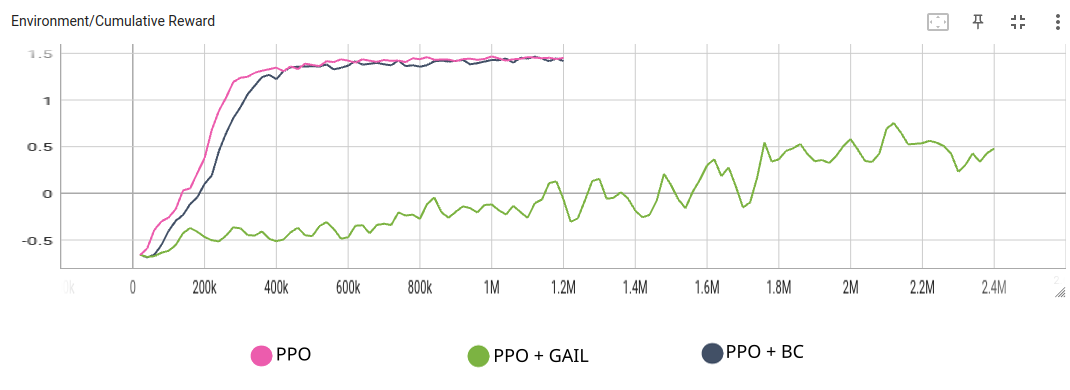
\includegraphics[scale=0.35]{figs/treinos/desafio-geral/recompensa-ppo-gail-bc.png}
    \caption{Recompensa cumulativa mediana por \textit{steps} durante o treino do agente em todos os trajetos.}
    \label{fig:result-desafio-geral}
\end{figure}

Nas tabelas \ref{resultado-tabela-geral-ppo}, \ref{resultado-tabela-geral-gail} e \ref{resultado-tabela-geral-bc} pode-se ver o detalhamento dos testes em cada rota dos algoritmos PPO, GAIL e BC, respectivamente. O \textit{Path(10)} mostrou-se como o trajeto mais difícil para PPO e BC, com a menor recompensa média nestes algoritmos e a segunda menor média no GAIL.

Interessante ressaltar que BC nestes testes conseguiu concluir o \textit{Path(3)} em todas as tentativas em contraste com o desafio anterior onde falhou em todas as dez tentativas, o que nos leva a crer que treinar em outros trajetos ajude o agente a cumprir um trajeto específico em vez de treinar somente em um único trajeto, pelo menos utilizando-se de Aprendizado por Imitação.

\begin{table}[htpb]
    \centering
    \caption{Detalhamento do desempenho no teste do desafio geral de PPO, inclui todas as tentativas, suas recompensas e a recompensa média por rota.}
    \label{resultado-tabela-geral-ppo}
    \begin{tabular}{|l|c|c|c|c|c|c|r|}
         \hline
         \multirow{2}{*}{Rota} & \multicolumn{2}{c|}{Tentativa 1}  & \multicolumn{2}{c|}{Tentativa 2} & \multicolumn{2}{c|}{Tentativa 3} & \multirow{2}{*}{Rec. Média} \\ \cline{2-7}
                               & \small{Concluiu?}  & \small{Rec.} & \small{Concluiu?} &\small{Rec.} & \small{Concluiu?} &\small{Rec.} &                               \\ \hline
            Path(0)   &      sim        &   1             &    sim          &      1        &    sim          &      1        &      1                 \\ \hline
            Path(1)   &      sim        &   1             &    sim          &      1        &    sim          &      1        &      1                 \\ \hline
            Path(2)   &      sim        &   1             &    sim          &      1        &    sim          &      1        &      1                 \\ \hline
            Path(3)   &      não        &   -0,18         &    sim          &      0,85     &    sim          &      1        &      0,56              \\ \hline
            Path(4)   &      sim        &   1             &    sim          &      1        &    sim          &      1        &      1                 \\ \hline
            Path(5)   &      sim        &   1             &    sim          &      0,8      &    sim          &      1        &      0,93              \\ \hline
            Path(6)   &      sim        &   1             &    não          &      -0,31    &    sim          &      1        &      0,56              \\ \hline
            Path(7)   &      sim        &   0,85          &    sim          &      1        &    sim          &      0,9      &      0,91              \\ \hline
            Path(8)   &      sim        &   1             &    sim          &      0,9      &    sim          &      1        &      0,96              \\ \hline
            Path(9)   &      sim        &   1             &    sim          &      0,95     &    sim          &      1        &      0,98              \\ \hline
            Path(10)  &      não        &   0,12          &    não          &      0,02     &    sim          &      1        &      0,38              \\ \hline
            Path(11)  &      sim        &   1             &    sim          &      1        &    sim          &      1        &      1                 \\ \hline
            Path(12)  &      sim        &   1             &    sim          &      1        &    sim          &      1        &      1                 \\ \hline
            Path(13)  &      sim        &   1             &    sim          &      1        &    sim          &      1        &      1                 \\ \hline
            Path(14)  &      sim        &   1             &    sim          &      1        &    sim          &      1        &      1                 \\ \hline
            Path(15)  &      sim        &   1             &    sim          &      1        &    sim          &      1        &      1                 \\ \hline
            Path(16)  &      sim        &   1             &    sim          &      1        &    sim          &      1        &      1                 \\ \hline
    \end{tabular}
\end{table}

\begin{table}[htpb]
    \centering
    \caption{Detalhamento do desempenho no teste do desafio geral de GAIL.}
    \label{resultado-tabela-geral-gail}
    \begin{tabular}{|l|c|c|c|c|c|c|r|}
         \hline
         \multirow{2}{*}{Rota} & \multicolumn{2}{c|}{Tentativa 1}  & \multicolumn{2}{c|}{Tentativa 2} & \multicolumn{2}{c|}{Tentativa 3} & \multirow{2}{*}{Rec. Média} \\ \cline{2-7}
                               & \small{Concluiu?}  & \small{Rec.} & \small{Concluiu?} &\small{Rec.} & \small{Concluiu?} &\small{Rec.} &                               \\ \hline
            Path(0)            &      sim          &   1          &    não            &      -0,677 &    sim            &      -0,402 &      -0,026                    \\ \hline
            Path(1)            &      não          &   0,231      &    não            &      -0,01  &    não            &      -0,253 &      -0,011                    \\ \hline
            Path(2)            &      não          &   -0,375     &    não            &      -0,153 &    não            &      -0,551 &      -0,36                     \\ \hline
            Path(3)            &      não          &   -0.412     &    não            &      0,002  &    não            &      -0,588 &      -0,333                    \\ \hline
            Path(4)            &      não          &   -0,086     &    sim            &      1      &    não            &      -0,504 &      0,137                     \\ \hline
            Path(5)            &      não          &   -0,278     &    não            &      0,132  &    não            &      -0,515 &      -0,22                     \\ \hline
            Path(6)            &      sim          &   1          &    sim            &      1      &    não            &      0,201  &      0,734                     \\ \hline
            Path(7)            &      não          &   -0,297     &    não            &      -0,22  &    não            &      -0,636 &      -0,384                    \\ \hline
            Path(8)            &      não          &   0,087      &    não            &      -0,087 &    não            &      0,215  &      0,072                     \\ \hline
            Path(9)            &      não          &   -0,084     &    não            &      0,204  &    não            &      -0,104 &      0,006                     \\ \hline
            Path(10)           &      não          &   -0,44      &    não            &      -0,677 &    não            &      -0,586 &      -0,566                    \\ \hline
            Path(11)           &      não          &   0,063      &    não            &      -0,182 &    sim            &      1      &      0,293                     \\ \hline
            Path(12)           &      não          &   0,074      &    não            &      -0,44  &    não            &      -0,655 &      -0,292                    \\ \hline
            Path(13)           &      nào          &   0,191      &    não            &      -0,686 &    não            &      -0,668 &      -0,718                    \\ \hline
            Path(14)           &      não          &   0,098      &    não            &      -0,644 &    não            &      -0,553 &      -0,366                    \\ \hline
            Path(15)           &      não          &   -0,579     &    não            &      -0,397 &    não            &      -0,47  &      -0,604                    \\ \hline
            Path(16)           &      sim          &   1          &    não            &      -0,665 &    não            &      -0,653 &      -0,106                    \\ \hline
    \end{tabular}
\end{table}

\begin{table}[htpb]
    \centering
    \caption{Detalhamento do desempenho no teste do desafio geral de BC.}
    \label{resultado-tabela-geral-bc}
    \begin{tabular}{|l|c|c|c|c|c|c|r|}
         \hline
         \multirow{2}{*}{Rota} & \multicolumn{2}{c|}{Tentativa 1}  & \multicolumn{2}{c|}{Tentativa 2} & \multicolumn{2}{c|}{Tentativa 3} & \multirow{2}{*}{Rec. Média} \\ \cline{2-7}
                               & \small{Concluiu?}  & \small{Rec.} & \small{Concluiu?} &\small{Rec.} & \small{Concluiu?} &\small{Rec.} &                               \\ \hline
            Path(0)   &      sim        &   1             &    sim          &      1        &    sim          &      1        &      1                 \\ \hline
            Path(1)   &      sim        &   1             &    sim          &      1        &    sim          &      1        &      1                 \\ \hline
            Path(2)   &      sim        &   1             &    sim          &      1        &    sim          &      1        &      1                 \\ \hline
            Path(3)   &      sim        &   1             &    sim          &      0,9      &    sim          &      1        &      0.967             \\ \hline
            Path(4)   &      sim        &   1             &    sim          &      1        &    sim          &      1        &      1                 \\ \hline
            Path(5)   &      sim        &   1             &    sim          &      1        &    sim          &      1        &      1                 \\ \hline
            Path(6)   &      sim        &   1             &    sim          &      1        &    sim          &      1        &      1                 \\ \hline
            Path(7)   &      sim        &   1             &    sim          &      0,95     &    sim          &      1        &      0,983             \\ \hline
            Path(8)   &      sim        &   1             &    sim          &      0,95     &    sim          &      1        &      0,983             \\ \hline
            Path(9)   &      sim        &   1             &    sim          &      1        &    sim          &      1        &      1                 \\ \hline
            Path(10)  &      não        &   0,224         &    não          &      0,158    &    não          &      0,221    &      0,201             \\ \hline
            Path(11)  &      sim        &   1             &    sim          &      1        &    sim          &      1        &      1                 \\ \hline
            Path(12)  &      sim        &   1             &    sim          &      1        &    não          &      -0,41    &      0,53              \\ \hline
            Path(13)  &      sim        &   1             &    sim          &      1        &    sim          &      1        &      1                 \\ \hline
            Path(14)  &      sim        &   1             &    sim          &      1        &    sim          &      1        &      1                 \\ \hline
            Path(15)  &      sim        &   1             &    sim          &      1        &    não          &      0,12     &      0,707             \\ \hline
            Path(16)  &      sim        &   1             &    sim          &      1        &    sim          &      1        &      1                 \\ \hline
    \end{tabular}
\end{table}

Por fim na Tabela \ref{resultado-tabela-desafio-geral}, temos o resultado consolidado geral dos testes deste desafio, onde é possível ver uma diferença muito grande entre GAIL e os demais. GAIL cumpriu apenas 7 dos 51 testes (aprox. 13,7\%), enquanto PPO e BC concluíram 47(92,1\%) e 46(90,2\%) dos 51 testes, respectivamente. 

\begin{table}[htpb]
    \centering
    \caption{Consolidado de resultados no desafio geral.}
    \label{resultado-tabela-desafio-geral}
    \begin{tabular}{|l|c|c|c|r|}
         \hline
         \small{Rota}           & \small{Algoritmo}   & \small{Mediana final rec. Treino}  & \small{Desempenho testes}    & \small{Média rec. Testes} \\ \hline
         \multirow{3}{*}{Todas} &      PPO            &   1,451                            &    47/51                     &      0,899                \\ \cline{2-5}
                                &      GAIL           &   0,479                            &    7/51                      &      -0,161               \\ \cline{2-5}
                                &      BC             &   1,416                            &    46/51                     &      0,904                \\ \hline
    \end{tabular}
\end{table}